%fichier : Projet_Di4_PPGL_Astie-Teddy.tex
%Date : 03/01/2023
%Version : 1.00

\documentclass{EPUProjetDi}
\usepackage{listings}

\makeindex

%remplir les lignes suivantes avec les informations vous concernant :
\title[Projet FourmiLaby Rust]{Serveur Rust pour le projet Labyrinthe de Fourmis}

\projet{Projet de Programmation et Génie Logiciel}

\author{Teddy Astie\\ %Attention : toujours écrire d'abord le prénom puis le nom (ne pas mettre tout le nom en majuscules)
\noindent[\url{teddy.astie@etu.univ-tours.fr}]\\
}

\encadrant{Nicolas Monmarché\\ %
\noindent[\url{nicolas.monmarche@univ-tours.fr}]\\~\\
Polytech Tours\\
Département Informatique\\~ %
}

%%%%%%%%%%%%%%%%%%%%%%%%%%%%%%%%%%%%%%%%%%%%%%%%%%%%%%%%%%%%%%%%%%%%%%%%%%%%%%%%%%%%%%%%%%
\begin{document}

\maketitle

\pagenumbering{roman}
\setcounter{page}{0}

{
%on réduit momentanément l'écart entre paragraphes pour ne pas trop aérer la table des matières
\setlength{\parskip}{0em}

\tableofcontents

%\listoffigures
%rq1 : si vous n'avez pratiquement pas de figures, laissez la ligne précédente en commentaire

%\listoftables
%rq1 : si vous n'avez pratiquement pas de tables, laissez la ligne précédente en commentaire
}


\start
%%%%%%%%%%%%%%%%%%%%%%%%%%%%%%%%%%%%%%%%%%%%%%%%%%%%%%%%%%%%%%%%%%%%%%%%%%%%%%%%%%%%%%%%%%

\chapter*{Introduction}
%le 2 lignes suivantes permettent d'ajouter l'introduction à la table des matières
%et d'afficher "Introduction en haut des pages"
\addcontentsline{toc}{chapter}{\numberline{}Introduction}
\markboth{\hspace{0.5cm}Introduction}{}

Ce projet fait partie de l'ensemble des projets du "jeu de fourmis" proposé par Nicolas Monmarché. Il en constitue notamment l'un des serveurs ici le serveur codé en Rust.

\section{Rappel du principe de jeu Labyrinthe de Fourmis}

Le jeu labyrinthe de fourmis est un jeu coopératif dont l'objectif est d'obtenir le plus de points en apportant de la nourriture jusqu'au nid au travers d'un labyrinthe. Afin de faciliter les décisions des joueurs, un mécanisme de phéromone est mis en place, afin de déterminer le chemin pris par un joueur qui a réussi à apporter la nourriture jusqu'au nid.

L'environnement de jeu est un labyrinthe sur une grille en 2 dimensions pour lequel chaque case peut comporter des mur dans chaque direction ainsi qu'éventuellement de la nouriture et/ou un nid. Le joueur doit trouver un chemin du nid jusqu'à une source de nourriture en tenant compte des murs, et si possible en prenant le plus court chemin.

Lorsque le joueur trouve de la nourriture, il émet des phéromones sur les cases qu'il traverse, jusqu'à ce qu'il arrive au nid.

Chaque joueur reçoit une copie du labyrinthe lors de son arrivée sur la partie, ainsi que régulièrement (chaque seconde) le niveau de phéromone de chaque case.

Le client et le serveur communiquent selon un protocole de communication basé sur du JSON et par du TCP/IP.

Le serveur est capable de gérer plusieurs parties en même temps, une phase de connexion/négociation est effectuée lorsque qu'un client se connecte au serveur, de plus, il est possible pour un joueur de se reconnecter à une partie après un éventuel problème de connexion (à l'aide de son UUID).

\section{Intérêt du langage Rust dans le projet}

Initialement, les langages proposés furent le C et éventuellement le C++. Toutefois, ce projet sous-entends tout un ensemble de problèmes difficiles à gérer dans ces langages : synchronisation, gestion mémoire, ... ce qui peut être grande source de difficultés (bugs, plantages, ...) en C ou même C++\footnote{bien que les standards modernes du type C++20 aident partiellement à résoudre ces problèmes mais au prix d'un code bien plus complexe et bien en dehors du cadre de nos cours de C++}.

\begin{center}
  
\includegraphics[width=\linewidth/2]{rust-social-wide.jpg}
\end{center}

Le langage Rust qui a gagné beaucoup d'intérêt ces dernières années est décrit comme un "langage de programmation fiable, concurrent, pratique" ayant un modèle de concurrence inspiré de l'Erlang\footnote{\url{https://www.erlang.org/}} et conçu pour produire des logiciels fiables et robustes tout en garantissant une très haute performance. Ce langage a été en grande partie conçu pour éviter une grande partie des problèmes cités au dessus (synchronisation, gestion mémoire) avec des mécanismes particuliers comme par exemple système d'ownership/borrowing strict, le paramètre de durée de vie (non utilisé dans le projet), divers marqueurs (comme \verb|MaybeUninit<T>|), clonage non implicite, etc. De plus, le directeur technique de Microsoft Azure nous recommande d'utiliser Rust à la place de C et C++ pour des nouveaux projets\cite{markrussinovich}.

Pour toutes ces raisons et d'autres encore, le langage Rust a été choisi pour réaliser ce projet.

\chapter{Structure générale du projet}

\begin{center}
  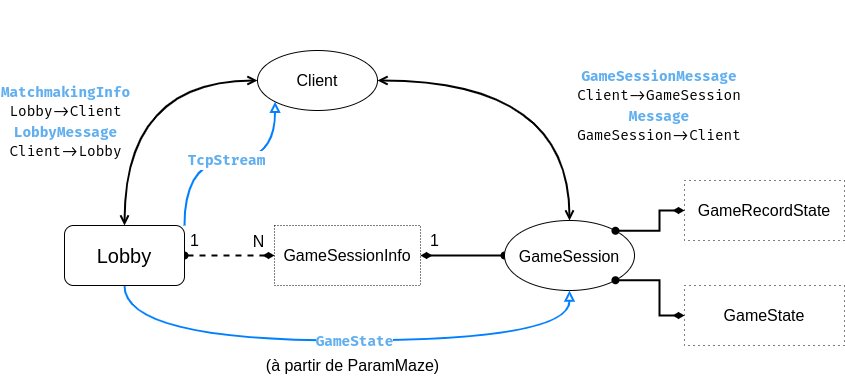
\includegraphics[width=\linewidth]{Diagramme structure.png}
  \label{fig:DiagrammeStructure}
  
  \includegraphics[width=\linewidth/2]{Légende diagramme structure.png}

  Organisation générale du projet (non exhaustif)
\end{center}

Le projet est divisé en divers composants (ou modules) intéragissants entre eux en utilisant des canaux asynchrones de type Multiple-Producer Single-Consumer disponibles dans la librairie standard Rust depuis le module \verb|syd::sync::mpsc|\footnote{\url{https://doc.rust-lang.org/std/sync/mpsc/index.html}}. Ce modèle s'apparente au modèle d'acteur\footnote{\url{https://fr.wikipedia.org/wiki/Modèle_d'acteur}} qui consiste à avoir plusieurs "acteurs" qui communiquent par passage de message, dans notre cas, hormis pour la gestion des \verb|GameSessionInfo| qui se fait par partage mémoire et comptage de référence (\verb|Arc<>| + \verb|Weak<>|), tout le reste communique par passage de message et instanciation de nouveaux acteurs.

Le projet comporte aussi d'autres parties plutôt utilitaires qui ne sont pas affichés dans le diagramme dont l'implémentation du protocole de communication (\verb|message|), l'intéraction avec la librairie de génération de labyrinthe (\verb|external::generator|) ou encore la gestion d'erreur (\verb|error|) et la structure de labyrinthe (\verb|maze|).

Le projet est relativement modulaire, et a été pensé pour être extensible (on peut par exemple ajouter des fonctionnalitées dans les modules en ajoutant de nouveaux types de message acceptés), ainsi qu'en essayant de décupler les objets en sous-objets (en particulier pour \verb|GameSession| découpé en objets plus pratiques pour implémenter certains traits (comme \verb|Serializable| pour \verb|GameState|)), ce qui peut nous permettre par exemple ici d'enregistrer l'état d'une partie dans un fichier.

\begin{center}
  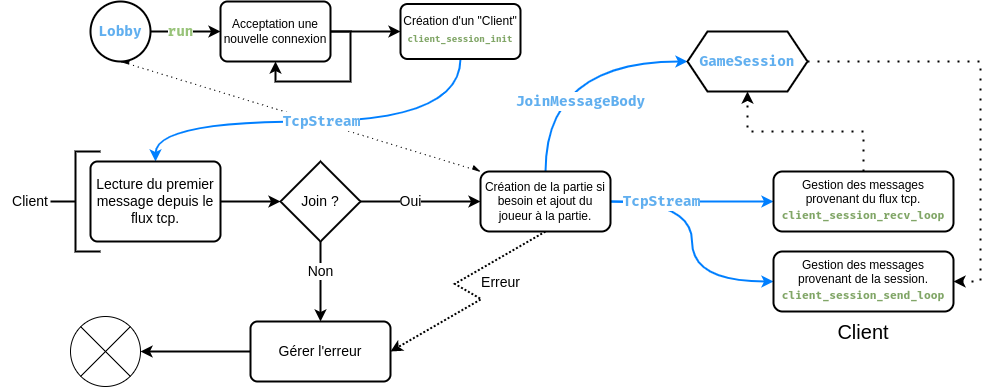
\includegraphics[width=\linewidth]{Diagramme flux.png}
  \label{fig:DiagrammeFlux}

  Flot d'exécution général
\end{center}

\chapter{Présentation des modules clés}

\section{Lobby}

L'exécution commence tout d'abord dans le \verb|Lobby| qui a deux responsabilitées.

Tout d'abord, le \verb|Lobby| accepte les différents sockets, et construit des clients.

En même temps (dans un thread à part), le \verb|Lobby| reçoit des messages de la part des clients pour trouver une partie (\textit{matchmaking}, en créant si besoin la partie), ainsi qu'effectuer d'autres tâches de maintenance des structures de données (supprimer les références vers des parties qui n'existent plus) et gère la liste des parties en cours, des liens entre les \verb|UUID| des joueurs et leur serveur associé.

\section{Client}

Le \verb|client| est construit par le \verb|Lobby| à partir du \verb|TcpStream| qui vient de se connecter, et d'un canal vers le \verb|Lobby|. La première étape du \verb|client| est de se charger de vérifier et rediriger la négociation d'une partie avec le \verb|Lobby| afin de se connecter à une \verb|GameSession|. Une fois le client connecté à la \verb|GameSession|, ce client se charge de vérifier et rediriger tous les \verb|Message| provenant du \verb|TcpStream| jusqu'à la \verb|GameSession| ainsi que tous les messages de la \verb|GameSession| jusqu'au \verb|TcpStream|.

En cas d'erreur fatale (message inattendu, JSON invalide, erreur réseau, plantage de la parties), envoie si possible une erreur au \verb|TcpStream|, stoppe le \verb|TcpStream| puis detruit le canal du client ce qui va à terme invalider la connexion du client pour la \verb|GameSession|.

\section{GameSession}

L'acteur \verb|GameSession| pilote une \verb|GameState| à partie des messages qu'il reçoit, notamment, il gère une liste de clients connectés, gère leur éventuelle déconnection. Il gère également l'évaporation régulière des niveaux de phéromones pour chaque case ainsi l'envoi régulier des niveaux de phéromones.
De plus, il détient la \verb|GameSessionInfo|.
Une fonctionnalité expérimentale gérée par le \verb|GameSession| est l'enregistrement automatique des parties par \verb|GameRecordState|.

\section{GameState}

La structure de \verb|GameState| est l'état instantanné de la partie, il détient toutes les informations sur l'état de la partie : le labyrinthe considéré, les niveaux de phéromones, les \verb|UUID| des joueurs, et leur position ainsi que si ils détiennent de la nouriture.
Par conséquent, le \verb|GameState| n'a aucune connaissance de si un certain joueur est actuellement connecté ou non et détient que des objets bruts dont des listes, le rendant notamment compatible avec les traits \verb|Clone|, \verb|Send| et \verb|Serializable|.

En plus de cela, cette structure implémente diverses méthodes pour gérer la logique du jeu (déplacements des fourmis, actualisation des niveaux de phéromones, actualisation de l'évaporation, etc.).

\section{GameRecordState et GameRecord}

La structure de \verb|GameRecordState| définit un état d'enregistrement, donc l'instant du dernier message (pour calculer les délais), les différents messages depuis le début de la partie, etc., il est utilisé pour construire à terme le \verb|GameRecord| qui est une version figée dans le marbre et \verb|Serializable| de \verb|GameRecordState|.

L'enregistrement d'une partie trace l'intégralité des messages envoyés par les joueurs, le labyrinthe considéré, ainsi que le moment auquel chaque message a été reçu, cela permet de rejouer une partie. Un mécanisme expérimental pour rejouer une partie existe dans le module \verb|client::record|.

\chapter{Choix techniques et apports du Rust}

\section{Système concurrent par passage de message}

Le choix technique le plus notable dans le projet, c'est d'utiliser une approche concurrente fonctionnant principalement par passage de message à l'inverse d'une approche plutôt orientée objet à mémoire partagée.

Cette approche est particulièrement pratique pour exploiter plusieurs processeurs tout en évitant tout un ensemble de problème de synchronisation que l'on pourrait avoir avec une autre approche. De cette manière, la modélisation obtenue s'apparente au modèle d'acteur\footnote{\url{https://fr.wikipedia.org/wiki/Modèle_d'acteur}}.

L'approche orientée objet fonctionnant exclusivement par partage mémoire aurait été limitée car chercher à rendre le code parallèle aurait été ardu comme cela aurait impliqué l'utilisation d'un grand nombre de \verb|Mutex| ainsi que d'autres outils de synchronisation donc aura compliqué plusieurs parties du code. Même en négligeant le parralèlisme donc n'utiliser qu'un unique thread, étant donné que l'on souhaite manipuler plusieurs sockets et plusieures sessions de jeu au même moment, on aurait eu d'une manière à implémenter tout un mécanisme de gestion d'I/O asynchrone ou utiliser une librairie pour le faire à notre place, ce qui est loin d'être simple. C'est pourquoi une approche évitant le couplage est plus souhaitable.

Le Rust nous offre un large panel d'outil pour implémenter les deux approches (passage de message et mémoire partagée), ce qui est pratique car on peut suivant ce que l'on souhaite effectuer, on peut choisir une approche au lieu d'une autre. Dans notre cas, l'ensemble du projet fonctionne par passage de message à l'exception des informations des parties qui est partagée entre le \verb|Lobby| et la \verb|GameSession| (afin notamment de pouvoir déterminer si la partie concernée est en cours ou non, à l'aide de la validité de la référence que détient le \verb|Lobby| vers cette structure).

Il est utile de noter que la plupart des librairies asynchrones Rust\footnote{async-std, tokio} favorisent une approche par passage de message avec par exemple des versions adaptées de \verb|std::sync::mpsc|.

\section{Garanties de fiabilité}

Le langage Rust met en oeuvre tout un ensemble de mécanisme ayant des implications sur le code pour éviter les fuites mémoires sans pour autant nécessiter un garbage-collector (bien qu'il soit possible d'en obtenir avec des références cycliques de \verb|Rc<T>|), d'accéder à des références invalides, certains problèmes liés à l'aliasing, les \textit{race conditions}, \dots Cela peut impliquer l'utilisation de types particulier pour encapsuler nos objets si l'on veut permettre à l'objet d'être référencé à plusieurs endroits (\verb|Rc<T>| et \verb|Arc<T>| similaires à \verb|std::shared_ptr| en C++) ou encore si l'objet peut être modifié par plusieurs thread (\verb|Mutex<T>|), etc\dots

Cela prend notamment la forme de \textit{traits} ($\approx$ interface) spécifiques indiquant si l'objet peut être transféré dans un autre thread ou encore partagée entre plusieurs threads\footnote{\url{https://doc.rust-lang.org/nomicon/send-and-sync.html}}.

De cette manière, un grand nombre d'éventuels problèmes de synchronisation ou de gestion mémoire sont évités ou simplifiés. Toutefois, ce fonctionnement est assez unique et pas très habituel dans d'autres langages de programmation, ce qui peut rendre compliqué l'apprentissage du Rust aux développeurs qui ne sont pas habitués à ces concepts.

\section{Traitement des messages à l'aide des \textit{tagged union} et du \textit{pattern matching}}

L'une des fonctionnalitées du langage Rust les plus pratiques pour implémenter le traitement des messages du protocole utilisé dans le jeu mais aussi ceux pour le passage de message est le pattern matching couplé aux \textit{tagged unions}\footnote{\url{https://en.wikipedia.org/wiki/Tagged_union}}\footnote{\url{https://doc.rust-lang.org/book/ch06-00-enums.html}}. Cet outil nous permet de créer des \textit{types somme} qui est une sorte d'énumération (plus précisément, une version améliorée des énumérations), mais dont chaque variant peut avoir des valeurs ou non (sous la forme d'une valeur, tuple, structure, ...). On peut par exemple définir un union taggué pouvant recevoir chaque type de message supporté par le protocole ainsi que leurs valeurs.

Cette fonctionnalité est également très utilisée dans les fonctionnalitées de base du langage, nottament \verb|Option<T>|\footnote{\url{https://doc.rust-lang.org/core/option/index.html}}, \verb|Result<T, E>|\footnote{\url{https://doc.rust-lang.org/core/result/index.html}}(gestion d'erreur), et bien d'autres.

\begin{center}
  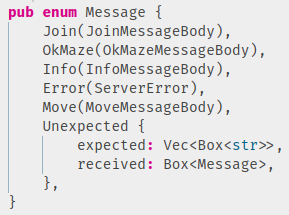
\includegraphics[width=\linewidth/3]{EnumMessage.png}
  \label{fig:EnumMessage}

  Enumeration pour les messages du protocole de communication
\end{center}

En utilisant \verb|match|, il est possible de prendre une décision pour chaque variant de l'union taggué/enumération, tout en destructurant chaque variant, ce qui permet de facilement utiliser ces objets. Il est également possible de faire du "pattern matching" à l'aide de match y compris sur l'élément à l'intérieur du match.

\begin{center}
  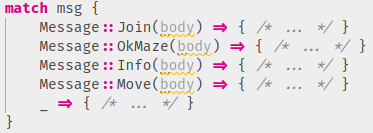
\includegraphics[width=\linewidth/2]{MatchMessage.png}
  \label{fig:MatchMessage}

  Utilisation de match sur un message suivant son type
\end{center}

Cette fonctionnalité est extensivement utilisée pour le traitement de message, que ce soit provenant d'un client distant (socket), ou pour le passage de messages entre les acteurs. Il existe une alternative dans le cas où seulement un seul cas particulier nous intéresse (\verb|if let|\footnote{\url{https://doc.rust-lang.org/book/ch06-03-if-let.html}})

\section{Sérialisation de données à l'aide de serde et serde-json}

Serde\footnote{\url{https://serde.rs/}} est un framework de sérialisation de donnéees Rust (ce framework fait parties de \url{https://blessed.rs}), il permet de rendre des types \verb|Serialize| et \verb|Deserialize| de manière automatiques (en utilisant \verb|derive|) ou non ainsi que personaliser la manière dont est structuré la donnée. En complément à cette librairie peut être implémenté une librairie pour sérialiser et désérialiser différents format de sérialisation, en particulier pour notre projet le format JSON à l'aide de \verb|serde-json|\footnote{\url{https://crates.io/crates/serde_json}}.

De cette manière, en utilisant \verb|serde-json|, on peut très facilement sérialiser ainsi que désérialiser l'ensemble des messages que peut envoyer ou recevoir le serveur, ce qui s'avère extrêmement pratique pour implémenter le protocole.

De plus, cela permet de facilement changer le format de sérialisation si nécessaire sans impliquer de grands changements dans le reste code.

\section{Gestion (quasi-)systématique des erreurs}

Certains langages de programmation, dont le C++ et le Java gèrent les erreurs par un mécanisme d'exception, d'autres comme le C utilisent une valeur de retour d'erreur pour indiquer d'une erreur est survenue.

Le langage Rust utilise principalement\footnote{bien qu'il existe un autre mécanisme de gestion d'erreur similaire aux exceptions pour des erreurs critiques \url{https://doc.rust-lang.org/book/ch09-01-unrecoverable-errors-with-panic.html}} une valeur de retour pour indiquer une erreur. Cela prend la forme d'un type \verb|Result<T, E>|\footnote{\url{https://doc.rust-lang.org/core/result/}} qui indique soit une valeur valide, soit une erreur et d'un autre type \verb|Option<T>|\footnote{\url{https://doc.rust-lang.org/core/option/}} pour des fonctions qui pourrait ne pas retourner de valeur (sans pour autant que ce soit une erreur). Un \verb|Result<T, E>| doit être obligatoirement utilisé, par exemple en utilisant \verb|match| pour définir le comportement en cas d'erreur ou avec une valeur, il est également possible d'utiliser l'opérateur \verb|?|\footnote{\url{https://doc.rust-lang.org/book/ch09-02-recoverable-errors-with-result.html}} pour remonter l'erreur comme valeur de retour à la fonction, ce qui permet d'une manière, "de simuler des exceptions".

De plus, de la même manière que pour définir des exceptions, on peut définir nos propres types d'erreurs, et ainsi "normaliser" les erreurs que l'on peut avoir dans le projet. En effet, dans notre projet, l'objet \verb|ServerError| qui est utilisé à cet fin implémente \verb|Serializable|, ce qui a permis de facilement mettre en place un mécanisme de transmission des erreurs au client.

Le système d'exception du Rust est très pratique, car il nous empêche d'ignorer silencieusement les erreurs (et par conséquent déclencher des comportements indéfinis) rend les origines des erreurs plus claires (l'opérateur \verb|?| indique que l'opération gère son erreur en la remontant), seules les fonctions retournant \verb|Result<T, E>| peuvent échouer, permet de gérer imédiatement les erreurs, sans nécessiter d'écrire de bloc \verb|try catch|, etc.

\section{Riche ensemble d'outil pour développer le projet}

Le Rust fournit un conséquent panel d'outil pour développer le projet\footnote{\url{https://www.rust-lang.org/fr/tools}}, en allant d'une installation simplifiée\footnote{\url{https://rustup.rs/}}, en passant par le confort dans l'utilisation avec un éditeur\footnote{\url{https://rust-analyzer.github.io/}} ainsi que plusieurs outils liés aux pratiques de génie logiciel (compilation et gestion des librairies\footnote{\url{https://doc.rust-lang.org/cargo/index.html}}, génération de pages de documentation comme avec Doxygen\footnote{\url{https://doc.rust-lang.org/rustdoc/index.html}}, vérification du code\footnote{\url{https://doc.rust-lang.org/stable/clippy/index.html}}, conventions d'écriture\footnote{\url{https://rust-lang.github.io/rustfmt/}}, tests unitaires\footnote{\url{https://doc.rust-lang.org/book/ch11-00-testing.html}}, sans oublier l'aide fournie le compilateur\footnote{\url{https://youtu.be/CJtvnepMVAU}}).

Cet ensemble d'outil est consistent et pratique sans nécessiter de lourde configuration. C'est une partie de ce qui fait le succès du langage d'après une analyse de The Overflow [StackOverflow]\cite{stackoverflowloverust}\cite{stackoverflowrustpopular}.

Une grande partie de ces outils ont été utilisés pour réaliser ce projet. Cela participe à l'amélioration de la qualité du code, à la fiabilité ainsi qu'à la performance dans certains cas. Cela permet également de mettre en pratique certaines pratiques de génie logiciel.

\chapter{Organisation du projet}

\section{Gestion du projet Rust}

Etant donné que le projet a été développé uniquement par moi même, il n'y a pas grand chose à noter quant à la gestion du projet. Une chose importante tout de même que j'ai pu remarquer est l'importance de régulièrement travailler sur le projet, afin d'éviter de tout faire à la fin. Dans mon cas, et comme le montre le dépôt git, le projet a été régulièrement et au fur et à mesure développé, toutefois j'ai remarqué que certains binômes de d'autres projets de génie logiciel ont eu des difficultées à gérer leur temps. Il faut donc rester sur cette approche de travail régulier pour les projets à venir.

\section{Gestion du méta-projet Labyrinthe de Fourmis}

Notre sujet, malgré que ce soit un projet effectué en binôme (ou monôme), était développé en partie en collaboration avec les autres groupes afin nos projets soient compatibles dans la mesure du possible. De cette manière, plusieurs réunions ont été organisées, afin de décider comment implémenter le projet, définir le protocole, la forme du labyrinthe, et ensuite définir de quelle manière collaborer pour ce projet, etc.

Toutefois, assez rapidement, certains groupes ont perdu le contact avec le projet, ce qui a compliqué la collaboration, et a entraîné à terme des divergences dans ce qui a été implementé\footnote{en particulier la divergence dans le protocole implémenté entre les serveurs Rust et C++}. De plus, cela complique l'accès à certains outils, comme par exemples les joueurs pour tester nos serveurs, et ainsi vérifier que nos implémentations du protocoles sont correctes (dans les deux sens). Pour les projets futurs\footnote{dont le projet collectif de S8}, il faudra être très attentif sur les autres personnes du groupe quant à la cohésion et insister plus encore que ce qui a été effectué pour ce méta-projet à ce que les autres participants ne perdent pas le fil.

Pour autant, une grande partie des projets\footnote{notamment le code source des serveurs et des générateurs de labyrinthes utiles aux serveurs} était hébergée sur le Gitlab de l'université\footnote{\url{https://scm.univ-tours.fr}}, afin de faciliter la collaboration entre les projets. Par exemple, j'ai pu intégrer la librairie C++ à mon projet à l'aide d'un submodule git\footnote{\url{https://git-scm.com/book/en/v2/Git-Tools-Submodules}} ce qui s'avère pratique pour intégrer la compilation de la librairie C++ dans mon projet (malgré d'éventuelles difficultées liés à la librairie standard C++ qui n'est pas intégrée de base à la compilation Rust).

%--------------------------------------------------------------------------------
\chapter*{Conclusion}
\addcontentsline{toc}{chapter}{\numberline{}Conclusion}
\markboth{Conclusion}{}

\label{sec:conclusion}

Tout d'abord, ce projet m'a permis de mettre en perspective toute la problèmatique de gestion de projet. En effet, ce projet a cherché à faire coopérer plusieurs groupes, autour d'un même plus grand projet, ce qui peut rapidement devenir compliqué, par exemple, il peut arriver que certains groupes "partent dans leur coin" et développent leur partie du projet de leur côté donc sans trop coopérer avec les autres. Cela explique l'importance d'effectuer des réunions afin de mettre au clair ce que l'on souhaite effectuer afin d'éviter des divergences ou incompréhensions dans ce qui est effectué.

Il est entièrement possible que les autres groupes du projet aient estimé qu'il s'agissait d'un projet plutôt "individuel" et donc ont involontairement préféré ne pas coopérer avec les autres, bien que ce ne soit pas l'esprit du projet.

Ensuite, ce projet a consitué un véritable exercice concrêt de programmation en Rust, ce qui m'a permis d'apprendre plus en pronfondeur le langage, ainsi que son écosystème. Bien que ce soit pas mon tout premier projet (même petit) en Rust, cela a été le plus grand et important que j'ai effectué depuis que j'ai commencé à apprendre le langage (environ depuis 3 ans). J'ai pu expérimenter avec de nombreuses parties de la librairie standard Rust, toutes les subtilitées de l'interfaçage avec le C, la sérialisation, bien d'autres choses mais surtout la programmation concurrente par passage de message.

Depuis le début de cette année universitaire, le langage Rust a gagné énormément d'intérêt dans de nombreux domaines, par exemple, il est desormais officiellement supporté par le noyau Linux\cite{rustlinux} avec un certain succès (driver open-source pour le GPU de l'Apple M1\cite{asahi}, OpenCL dans Mesa3D\cite{rusticl}, et plus encore\cite{nvmerust}). De plus, le Rust intéresse de plus en plus les entreprises (CEA, Thales, AtoS, ...) et intéresse aussi bien le domaine de l'embarqué, que celui des services web, serveurs, librairies système, etc.

Etant donné que mon expérience avec ce langage fut extrêmement positive, je n'hésiterais pas à effectuer un stage autour du langage Rust, ce qui est de plus en plus proposé, et que les candidats pour ce genre de stage se font rares\footnote{hormis pour un stage promosé par AtoS explicitément prévus pour des novices du Rust qui intéresse beaucoup de candidats}.

%--------------------------------------------------------------------------------
%exemple de bibliographie
\begin{thebibliography}{99}
\label{sec:biblio}
\bibitem{markrussinovich} \url{https://www.zdnet.com/article/programming-languages-its-time-to-stop-using-c-and-c-for-new-projects-says-microsoft-azure-cto/}
\bibitem{stackoverflowloverust} \url{https://stackoverflow.blog/2020/06/05/why-the-developers-who-use-rust-love-it-so-much/}
\bibitem{stackoverflowrustpopular} \url{https://stackoverflow.blog/2020/01/20/what-is-rust-and-why-is-it-so-popular/}
\bibitem{rustlinux} \url{https://www.zdnet.com/article/linus-torvalds-rust-will-go-into-linux-6-1/}
\bibitem{asahi} \url{https://asahilinux.org/2022/11/tales-of-the-m1-gpu/}
\bibitem{rusticl} \url{https://www.phoronix.com/news/Rusticl-2022-XDC-State}
\bibitem{nvmerust} \url{https://lpc.events/event/16/contributions/1180/attachments/1017/1961/deck.pdf}
\end{thebibliography}


%--------------------------------------------------------------------------------
%si on donne des annexes :
\appendix
\addcontentsline{toc}{part}{\numberline{}Annexes}

%--------------------------------------------------------------------------------

\chapter{Liens utiles\label{sec:liens_utiles}}
Voici une petite liste d'url intéressantes au sujet de ce projet :

\begin{itemize}
\item Gitlab du projet \url{https://scm.univ-tours.fr/21906867t/serveur-fourmi}
\item Site officiel du Rust \url{https://www.rust-lang.org/fr/}
\item Référentiel de documentation Rust \url{https://www.rust-lang.org/fr/learn}
\item Référence en magie noire en Rust \url{https://doc.rust-lang.org/nomicon/}
\item Documentation de serde \url{https://serde.rs}
\end{itemize}




%--------------------------------------------------------------------------------
%index : attention, le fichier dindex .ind doit avoir le même nom que le fichier .tex
%\printindex

%--------------------------------------------------------------------------------
%page du dos de couverture :

\resume{Le méta-projet de jeu de fourmis est un jeu de simulation de fourmis multijoueur utilisant une architecture Client-Serveur. Ce projet propose une implémentation du serveur dans le langage Rust, et permet ainsi de mesurer l'intérêt de ce langage pour ce projet. Il fait partie avec le projet C++ des 2 implémentations du serveur pour ce jeu. }

\motcles{Rust, Simulation, Fourmis, Programmation Concurrente, Programmation Fonctionelle, Multithreading, Réseau, Sérialisation, Jeu, TCP}

\abstract{The meta-project of "ant simulation game" is a multiplayer ant simulation serious-game based on a Client-Server architecture. This project offer a Rust implementation for the server, and highlights the benefits of this programming language in this project. It is along with the C++ project one of the implementations of the server for this game.}

\keywords{Rust, Simulation, Ant, Concurrent Programming, Functionnal Programming, Multithreading, Network, Serialization, Game, TCP}

\makedernierepage


\end{document}
%%FIN du fichier